\documentclass[a4paper]{article}
\usepackage{array}
\usepackage[utf8]{inputenc}
\usepackage{float}
\usepackage[T1]{fontenc}
\usepackage[magyar]{babel}
%\usepackage{hyperref}
\usepackage{graphicx}
\usepackage{hhline}
\usepackage{amsmath}
\usepackage{amssymb}
\usepackage{mathtools}
\usepackage{anysize}
\marginsize{2.5cm}{2.5cm}{2.5cm}{2.5cm}


\begin{document}

\begin{titlepage}
	\begin{center}
		\vspace{1 cm}
		\Huge{\textbf{12. tétel: Rugó rezgései, leejtett rugó\\ }}
		\vspace{5 cm}
		\Large{Készítette: Kormányos Hanna Rebeka\\
				Dr. Groma István előadása alapján\\ 
				2018. tavasz}
	\end{center}
	
\end{titlepage}



\section*{Rugó rezgései}
Ebben a tételben egy súlyos rugóra akasztott test gravitációs térben való mozgását vizsgáljuk. \\
Tekintsünk egy $m$ tömegű rugóra akasztott $M$ tömegű testet ($M>>m$). Használjuk azt a modellt, miszerint a rugót egy rugalmas kontinuum (folytonos, szilárd közeg) , tehát nem "látjuk" a meneteit. \\
Legyenek a következő mennyiségek ismertek: $m$ a kontinuum tömege, $\rho$ a kontinuum sűrűsége, $A$ a kontinuum keresztmetszete, $L$ a kontinuum hossza, $M$ a kontinuumra akasztott test tömege, $g$ a nehézségi gyorsulás és $E$ a Young-modulus.\\ \\
A derékszögű koordinátarendszerünk origóját helyezzük a felfüggesztési pontba, valamit az $x$ tengely a gravitációs erővel legyen azonos irányítottságú. \\ 
A számolás során tekintsünk el a kontinuum harántirányú összehúzódásától, így ezen közelítés mellett $\underline{u}$-nak csak $x$ irányú komponense lesz, amit jelöljünk $u_{x}(x,t)$-vel mutatva, hogy az $x$ koordinától és az időtől függ.\\
Az előzőek alapján a feszültségtenzornak csak {xx} komponense lehet, ami arányos $u_x$ x szerinti deriváltjával, ahol az arányossági tényező $E$ (Young-modulus), hiszen itt egyszerű nyújtásról van szó. \\
$$

\subsubsection*{Mozgásegyenlet}
A kontinuumra a mozgásegyenlet ebben az esetben a következőképpen néz ki:\\

\begin{equation}
\label{}
\rho \cdot\frac{\partial^{2} u}{\partial t^{2}}=E \cdot \frac{\partial^{2} u}{\partial x^{2}}+\rho g
\end{equation}
\\
Ennek a\ differenciálegyenletnek így nincsen egyértelmű megoldása, meg kell még adnunk határfeltételeket.

\subsubsection*{Határfeltételek}
A kontinuum legfelső rögzített részére: \\

\begin{equation}
\underline{u}(0,t)=0
\end{equation}
\\
A kontinuum legalsó végére, amihez közvetlenül kapcsolódik az $M$ tömegű test: \\ 

\begin{equation}
\left M \cdot\frac{\partial^{2} u}{\partial t^{2}} \right|_{\mathrlap{L}}=\left Mg- AE \cdot \frac{\partial u}{\partial x} \right|_{\mathrlap{L}} 
\end{equation}

% $ \left  a\right|_{\mathrlap{V,N}}$ --- függőlegesvonal

\subsubsection*{Diff. egyenlet megoldása}
Alkalmazzunk egy trükköt, amit a múlt félévben mechanika előadáson láttunk. Bontsuk fel  $\underline{u}$-t 2-t komponensre. Legyen az egyik $u_{\infty}(x)$, ami nem függ az időtől és  $\tilde{u}(x,t)$, ami függ az időtől. \\
$u_{\infty}(x)$ meghatározható abból, hogy neki csak a statikus egyenletet kell kielégítenie,

\begin{equation}
\label{}
0=E \cdot \frac{\partial^{2} u_{\infty}}{\partial x^{2}}+\rho g
\end{equation}
\\
a következő $u_{\infty}$-re vonatkozó határfeltételekkel: \\

\begin{equation}
u_{\infty}(0)=0
\end{equation}

\begin{equation} 
\left  0=Mg-AE \cdot \frac{\partial u_{\infty}}{\partial x}\right|_{\mathrlap{L}}
\end{equation} 

\\
Vegyük észre, hogy ezt már megoldottuk 4. tételben (emlékeztető: parabola alakú megoldást kaptunk). 
\\
Mi jön ki $\tilde{u}$-ra?

\subsubsection*{$\tilde{u}$-ra vonatkozó egyenletek}
\\
$u_{\infty}$-re vonatkozó statikus egyenletet felhasznáva adódik:

\begin{equation}
\label{}
\rho \cdot\frac{\partial^{2} \tilde{u}}{\partial t^{2}}=E \cdot \frac{\partial^{2} \tilde{u}}{\partial x^{2}}-E \cdot \frac{\rho g}{E}+\rho g
\end{equation}
\\

\begin{equation}
\label{}
\frac{\partial^{2} \tilde{u}}{\partial t^{2}}=\frac{E}{\rho} \cdot \frac{\partial^{2} \tilde{u}}{\partial x^{2}}
\end{equation}
\\
Vezessük be a következő jelölést:
\begin{equation}
\label{}
c^{2}=\frac{E}{\rho}
\end{equation}
\\
Ekkor $\tidle{u}$-ra egy egyszerű hullámegyenlet adódik, tehát a feladatunk egy közönséges hullámegyenlet megoldása a következő határfeltételekkel:
\begin{equation}
\tilde{u}(0,t)=0
\end{equation}

\begin{equation} 
\left M \cdot \frac{\partial^{2} \tilde{u}}{\partial x^{2}}\right|_{\mathrlap{L}}=\left -AE \cdot \frac{\partial \tilde{u}}{\partial x}\right|_{\mathrlap{L}}
\end{equation} \\
\\
\subsubsection*{$\tilde{u}$ meghatározása}
\\
A rugó megnyúlik a saját és az $M$ tömegű test súlyától, de ekkor még nyugalomban van . E körül az egyensúlyi helyzet körül fog "mozogni" a test (kitérítés hatására), de azt hogy ez milyen fajta mozgás lesz csak az $\tilde{u} $-ra megoldott egyenlet adja meg.
\\
\\
Keressük a megoldást állóhullám formájába:
\begin{equation}
\tilde{u}(x,t)=u_{0} \cdot \sin(\omega t)\sin(kL)
\end{equation}
\\
Behelyettesítve a $(8)$ egyenletbe adódik:
\begin{equation}
- \omega^{2} \tilde{u}=- \frac{E}{\rho}k^{2} \tilde{u}
\end{equation}
\\
\begin{equation}
\omega^{2} =\frac{E}{\rho}k^{2}
\end{equation}
\\
Használjuk még ki a $(11)$ egyenletet:
\begin{equation}
-\omega^{2}M u_0 \sin(\omega t) \sin(kL)=-AEk \sin(\omega t) \cos(kL)
\end{equation}

\begin{equation}
-\omega^{2}M\sin(kL)=AEk \cos(kL)
\end{equation}
\\
Még egy egyenletet kaptunk $k$-ra, $\omega$-ra, amibe behelyettesítve a $\omega^{2} =\frac{E}{\rho}k^{2}$ összefüggést adódik:

\begin{equation}
\frac{E}{\rho} k^{2} M \sin(kL)=AEk \cos(kL)
\end{equation}
\\
Innen:
\begin{equation}
\frac{M}{\rho A L} kL =\ctg(kL)
\end{equation}
\\
Vegyük észre, hogy $\rho A L=m$ és vezessük be a $kL=x$ jelölést, ekkor adódik:
\begin{equation}
\frac{M}{m} x= ctg(x)
\end{equation}
\\
A kapott egyenletet grafikusan egyszerűen meg tudjuk oldani. Láthatjuk, hogy
végtelen sok megoldás van $x$-re. Ám a csillapodás miatt csak a legkisebb frekvenciájú rezgés marad meg, tehát csak az első metszéspontot vesszük figyelembe. Mivel $M >> m$, a lineáris egyenes meredeksége
nagyon nagy, ezért a kotangens függvényt kis x értékben fogja
metszeni. Ha x kicsi, akkor ctg(x)-et sorba fejthetjük a következő módon:
\begin{equation}
ctg(x) \approx \frac{1}{x}-\frac{x}{3}
\end{equation}
\\
(19) egyenletbe behelyettesítve adódik:
\begin{equation}
\frac{M}{m} x= \frac{1}{x}-\frac{x}{3}
\end{equation}
\\
\begin{equation}
\frac{M}{m} +\frac{1}{3}= \frac{1}{x^{2}}
\end{equation}
\\

\begin{equation}
M+\frac{m}{3} = \frac{m}{(kL)^{2}}
\end{equation}
\\
\begin{equation}
M+\frac{m}{3} = \frac{\rho L A}{\omega^{2} \frac{\rho}{E} L^{2}}
\end{equation}
\\
Végül $\omega^{2}$-re adódik a következő:
\begin{equation}
\omega^{2}=\frac{\frac{EA}{L}}{M+\frac{m}{3}}=\frac{D}{M+\frac{m}{3}}
\end{equation}
\\
Tehát sikerült levezetnünk a rugón kialakuló rezgések frekvenciáját $ M >> m $ esetben. Ez az összefüggés azt mondja, hogy a jelenséget tekinthetjük úgy, mintha egy súlytalan rugóra $M+\frac{m}{3}$ tömegű testet akasztottunk volna, ahol a $\frac{m}{3}$-at a rugó effektív tömegének nevezzük.

\section*{Leejtett rugó}
\\
A tétel második felében egy saját súlya alatt megnyúlt rugót engedünk el gravitációs térben, ennek a mozgását szeretnénk felírni.
\\
A mozgásegyenlet most is ugyanaz, mint a tétel 1. részében:

\begin{equation}
\label{}
\rho \cdot\frac{\partial^{2} u}{\partial t^{2}}=E \cdot \frac{\partial^{2} u}{\partial x^{2}}+\rho g
\end{equation}
\\
Most is úgy keressük a megoldást, hogy az  $\underline{u}$-t felbontjuk 2-t komponensre (az egyik $u_{\infty}(x)$, ami nem függ az időtől és  $\tilde{u}(x,t)$, ami függ az időtől).
\\ 
$u_{\infty}(x)$ meghatározható abból, hogy neki csak a statikus egyenletet kell kielégítenie:

\begin{equation}
\label{}
0=E \cdot \frac{\partial^{2} u_{\infty}}{\partial x^{2}}+\rho g
\end{equation}
\\
Vagyis:
\begin{equation}
\label{}
\frac{\partial^{2} u_{\infty}}{\partial x^{2}}=- \frac{\rho g}{E}
\end{equation}
\\
Ebből adódik $\tilde{u}(x,t)$, hogy:
\begin{equation}
\label{}
\rho \cdot \frac{\partial^{2} \tilde{u}}{\partial t^{2}}=E \cdot \frac{\partial^{2} \tilde{u}}{\partial x^{2}}
\end{equation}
\\
Ennek (28) a megoldása már a korábbiakból ismert:
\begin{equation}
\label{}
\underline{u}_{\infty}(x)=a+b\cdot x-\frac{\rho g}{2E} x^{2}
\end{equation}
\\
\\Viszont a határfeltételek most részben változni fognak, a következőképpen:

\begin{equation}
\label{}
u_{\infty}(0)=0
\end{equation}

\begin{equation}
\label{}
\left \frac{d u_{\infty}}{dx}\right|_{\mathrlap{L}}=0
\end{equation}
\\
\begin{equation}
\label{}
\left \frac{\partial \tilde{u}}{\partial x}\right|_{\mathrlap{L}}=0
\end{equation}
\\
\\
Ezekből a határfeltételekből (31) és (32) adódik, hogy $a=0$ és $b=\frac{\rho g}{E} \cdot L$
\\
Tehát:
\begin{equation}
\label{}
\underline{u}_{\infty}(x)=\frac{\rho g}{E} L \cdot x-\frac{\rho g}{2E} x^{2}=\frac{\rho g}{E} (L-\frac{x}{2})
\end{equation}
Innen kaphatunk még egy határfeltételt:
\begin{equation}
\label{}
\left \frac{d u_{\infty}}{dx}\right|_{\mathrlap{0}}=\frac{\rho g}{E} L
\end{equation}
\\
Az $x=0$ helyre (tehát a rugó legfelső pontjára) minden pillanatban igaz, hogy ott a feszültség 0. \\
(A $\sigma$-ban mind $u_{\infty}$ mind $\tilde{u}$ benne van.)
\begin{equation}
\label{}
\sigma (0,t)=0
\end{equation}
Ebből következik:
\begin{equation}
\label{}
\frac{d}{dx}(u_{\infty} + \tilde{u})(0,t)=0
\end{equation}
Így a fenti egyenlet csak akkor teljesül ($(35)$-ös egyenletet felhasználva), ha:
\begin{equation}
\label{}
\left \frac{d \tilde{u}}{dx}\right|_{\mathrlap{0}} =- \frac{\rho g}{E}L
\end{equation}
\\
$c^{2}=\frac{E}{\rho}$-t bevezetve az általános megoldás a következőképpen néz ki:
\begin{equation}
\label{}
f(x-ct)
\end{equation}
\\
Terjesszük ki $f$-et a $-x$ tartományban egy egyenessel, aminek a meredeksége $- \frac{\rho g}{E}L$. Az időben ez a görbe vonal csúszik az $x$ tengely mentén pozitív irányban $c$ sebességgel, amíg el nem éri az $L$ helyet a görbe "csúcsos" része. \\
Innen látható, hogy a rugó zuhanása közben a legalsó pont tényleg mozdulatlan lesz, amíg a rugó többi része "oda nem ér".
\\
\begin{figure}[!h]
	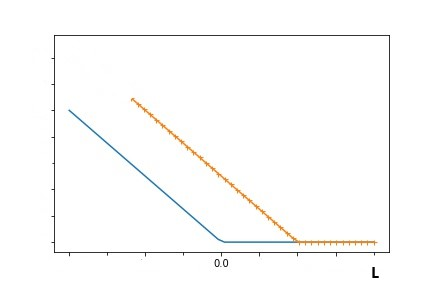
\includegraphics[height=7cm]{./plot3.jpg}
	\centering
%	\caption{Feszültség egyszerű nyújtás során deformáció függvényében (konstitúció).}
	\label{fig:abra}
	\end{figure}
\end{document}

